\section{Datasets}
\subsection{NTU Hand Dataset}
\noindent
The NTU hand dataset is primarily used to evaluate the hand pose estimation model \cite{handgcn}. This dataset is synthetically generated and provides annotations for 3D pose and 3D meshes \cite{handgcn}. Photorealistic textures and shape blending are applied on the hand model \cite{handgcn}. The dataset contains 500 common hand gestures captures from 1000 angles under 30 lightlights \cite{handgcn}. The dataset also contains hand of 5 skin colors and the images are composed with random backgrounds \cite{handgcn}. There are 315000 images for training and 60000 for testing \cite{handgcn}. 

\noindent
Figure \ref{fig:ntu_sample_data} shows a sample data from the NTU hand dataset. Although the image is synthetically generated, the hand is very realistic. This project removed the images where the palm faces away from the camera or the finger joints are mostly occluded. This is to reduce the network size to limit support for hand poses where the anchor points, such as the finger joints, are visible to some extent. 

\begin{figure}[ht]
    \begin{center}
        \begin{subfigure}[b]{0.35\textwidth}
            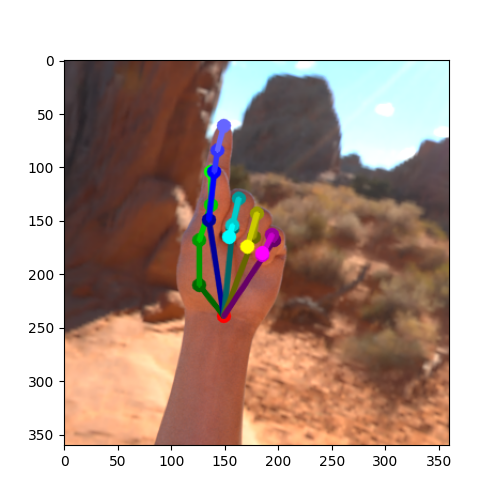
\includegraphics[width=150px]{assets/ntu_pose_2d.png}
            \caption{Pose 2D}
            \label{fig:ntu_pose_2d}
        \end{subfigure}
        \begin{subfigure}[b]{0.35\textwidth}
            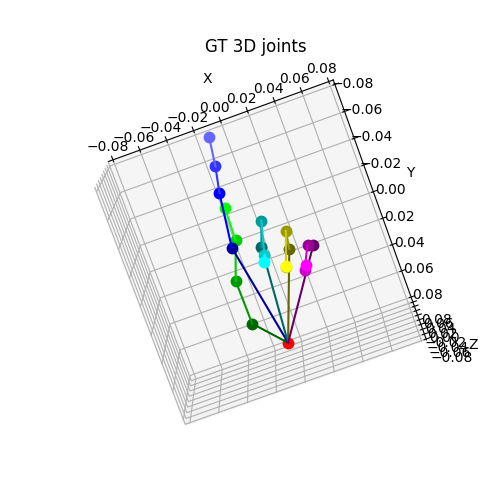
\includegraphics[width=150px]{assets/ntu_pose_3d.png}
            \caption{Pose 3D}
            \label{fig:ntu_pose_3d}
        \end{subfigure}
	    \caption{NTU Hand Data Sample}
	    \label{fig:ntu_sample_data}        
    \end{center}
\end{figure}

\newpage
\subsection{FreiHand Dataset}
\noindent
The Freihand is also used to evaluate the hand pose estimation model on real hands \cite{freihand}. A multi-view camera setup was setup to collect the hand poses and images without markers \cite{freihand}. The hand poses was collected from 32 subjects of different genders and ethic backgrounds, and they were tasked to perform actions with and without grasping objects \cite{freihand}. The hand poses were initially manually annotated, and a 3D model was trained on the existing dataset to predict and accelerate the fitting and annotation process \cite{freihand}.

\noindent
Figure \ref{fig:freihand_sample_data} shows a sample data from freihand dataset. The images were taken indoor and outdoor since the multi-view camera setup was portable \cite{freihand}. The images taken indoors were taken with a green background and augmented with random background by replacing the green pixels \cite{freihand}. This project removed the background augmented pictures because it does not generalises well to the outdoor images when the 2D pose estimation model was trained.
\begin{figure}[ht]
    \begin{center}
        \begin{subfigure}[b]{0.35\textwidth}
            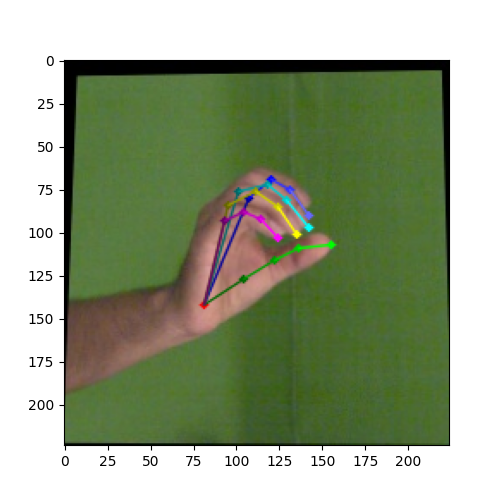
\includegraphics[width=150px]{assets/freihand_pose_2d.png}
            \caption{Pose 2D}
            \label{fig:freihand_pose_2d}
        \end{subfigure}
        \begin{subfigure}[b]{0.35\textwidth}
            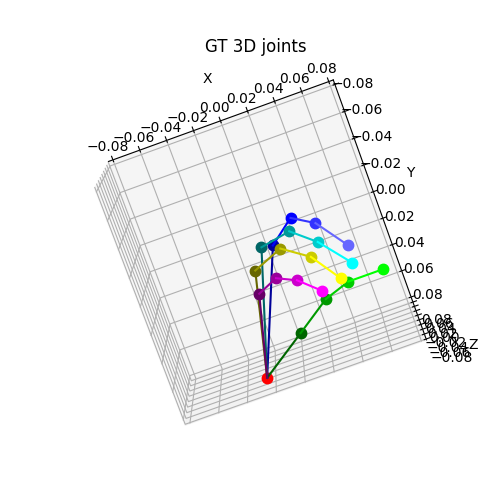
\includegraphics[width=150px]{assets/freihand_pose_3d.png}
            \caption{Pose 3D}
            \label{fig:freihand_pose_3d}
        \end{subfigure}
	    \caption{Freihand Data Sample}
	    \label{fig:freihand_sample_data}        
    \end{center}
\end{figure}


\newpage
\subsection{Custom Upper Body Dataset}
\noindent
An upper body pose estimation model is trained to provide the 3D position for the end effector of the robot. The pose estimation model is trained and evaluated on a custom dataset that was collected using a depth camera - Intel Realsense D455. The setup is shown in Figure \ref{fig:body_pose_data_collection_setup}. The distance from the joint to the camera is obtained from the depth image.

\begin{figure}[ht]
	\begin{center}
		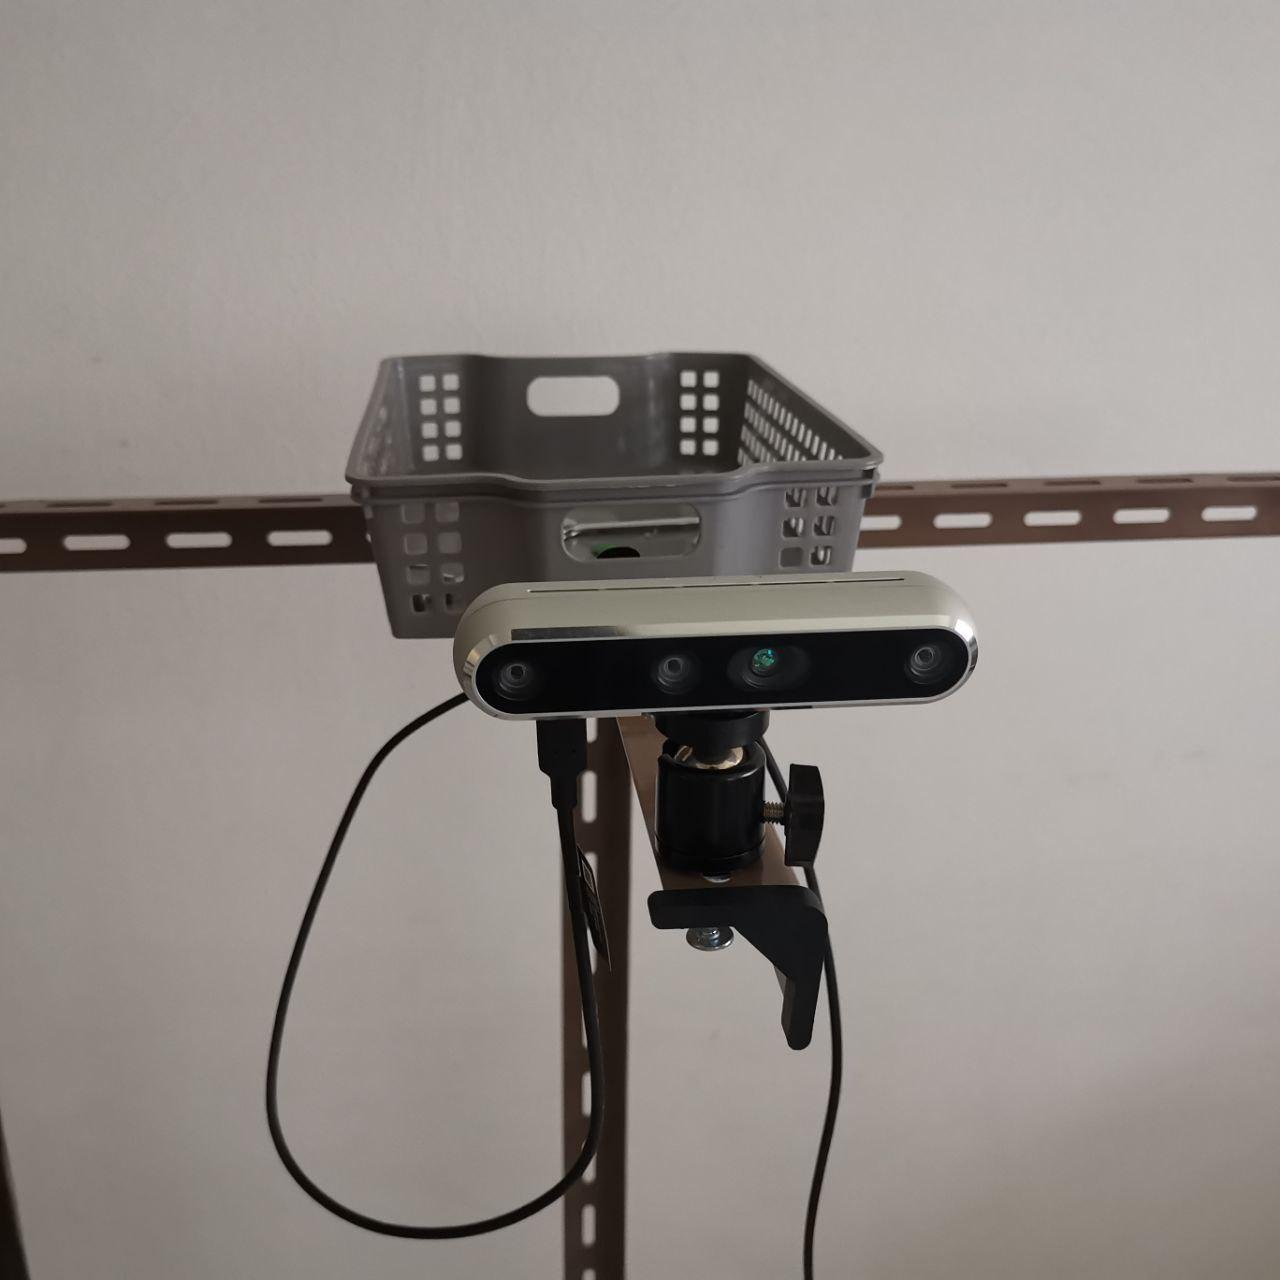
\includegraphics[width=100px]{assets/body_pose_setup.jpg}
		\caption{Body Pose Data Collection Setup}
		\label{fig:body_pose_data_collection_setup}
	\end{center}
\end{figure}

\noindent
Figure \ref{fig:custom_sample_data} shows a sample data of the upper body pose dataset. A lightweight pose 2D estimation model inferred the 2D keypoints to obtain the pixel coordinate \cite{lightweightopenpose}. The 3D pose was computed from the measured depth and camera intrinsic. If the depth image failed to measure the distance or the keypoints are occluded, the nearest pixel with a valid depth is searched. The data is collected for 10 different actions, and 3 different background for training and 2 different background for testing. There are 90000 images for training and 10000 for testing.

\begin{figure}[ht]
    \begin{center}
        \begin{subfigure}[b]{0.35\textwidth}
            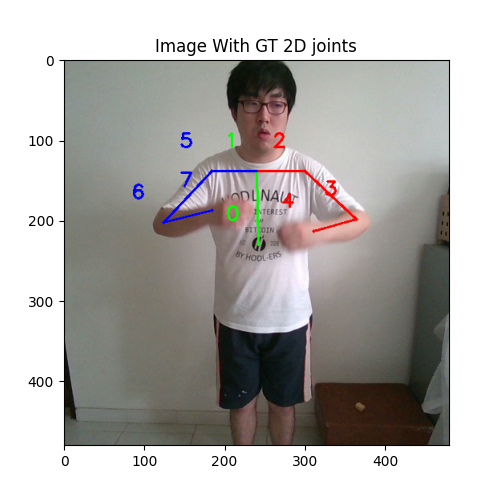
\includegraphics[width=150px]{assets/custom_pose_2d.png}
            \caption{Pose 2D}
            \label{fig:custom_pose_2d}
        \end{subfigure}
        \begin{subfigure}[b]{0.35\textwidth}
            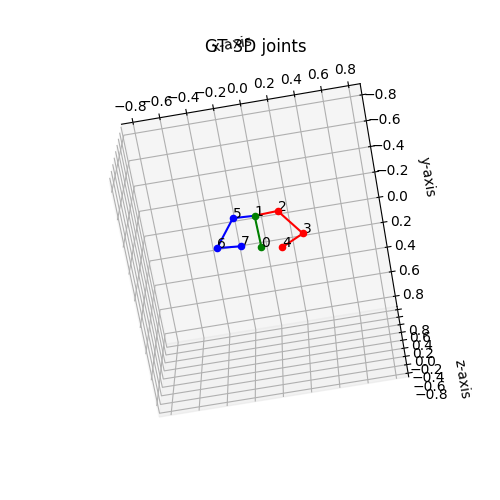
\includegraphics[width=150px]{assets/custom_pose_3d.png}
            \caption{Pose 3D}
            \label{fig:custom_pose_3d}
        \end{subfigure}
	    \caption{Custom Upper Body Data Sample}
	    \label{fig:custom_sample_data}        
    \end{center}
\end{figure}
